\documentclass[10pt,a4paper]{article}
\usepackage[T2A]{fontenc}    
\usepackage[english]{babel}   
\usepackage{color}
\usepackage[urlbordercolor={1 1 1},colorlinks=true]{hyperref}
\usepackage{longtable}
\usepackage{graphicx}
\usepackage[a4paper,left=2.5cm,right=2cm,top=2cm,bottom=2cm]{geometry}

\usepackage{mathptmx}
\usepackage{arev}
\usepackage{indentfirst}


%\input{newcommands}
\definecolor{link}{rgb}{0,0,0.6}

\hypersetup
{
	linkcolor=link,
	urlcolor={link}
}

\newcommand{\lmpratio}{0.15}
\newcommand{\rmpratio}{0.74}
\newcommand{\verticalSpace}{0.3cm}
\newcommand{\vSpace}{0.5cm}
\newcommand{\horizontalSpace}{0.05\textwidth}

\newcommand{\sectionTitle}[1]{\Large{\textbf{#1}}}
\newcommand{\sectionMain}[1]{\textbf{#1}}

\newcommand{\vacancyName}{PhD student}
\renewcommand*\familydefault{\sfdefault}
% \renewcommand{\familydefault}{\sfdefault}


\setlength{\parindent}{3em}
\setlength{\parskip}{0.5em}

\begin{document}

	\pagenumbering{gobble} 
	

	\raggedright{\Large{\textbf{Arseniy Shchepetnov}}}\\[0.3cm]
	
	\begin{minipage}[t]{0.8\textwidth}
		\vspace{0pt}
		\raggedright{\textbf{Data Science, Machine Learning Engineer, Data Engineer}}\\[0.3cm]
		% 	\raggedright{\huge\vacancyName}\\[0.3cm]
		% 	\noindent Date of birth: $15^{\mathrm{th}}$ December $1989$ \\[0.1cm]
		\noindent Address: Tbilisi, Georgia \\[0.1cm]
		\noindent Email: \href{mailto:a.shchepetnov@gmail.com}{a.shchepetnov@gmail.com}\\[0.1cm]
		\noindent GitHub: \href{https://github.com/ArseniyShchepetnov}{https://github.com/ArseniyShchepetnov}\\
            \noindent LinkedIn: \href{https://www.linkedin.com/in/arseniy-shchepetnov/}{https://www.linkedin.com/in/arseniy-shchepetnov/}\\
            \noindent Medium: \href{https://medium.com/@a.shchepetnov}{https://medium.com/@a.shchepetnov} \\
            \noindent Personal website: \href{https://arseniyshchepetnov.github.io/personal-website/}{https://arseniyshchepetnov.github.io/personal-website/}
	\end{minipage}
	% \begin{minipage}[t]{0.2\textwidth}
	% 	\vspace{0pt}
	% 	% 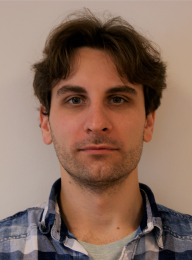
\includegraphics[width=\linewidth]{photo.png}
	% \end{minipage}

 
\vspace{\vSpace}

\begin{minipage}[t]{1\textwidth}
\vspace{0pt}
\quad My skill set covers full-cycle research and development of AI products. I created different parts of the AI production path: data infrastructure, training and deployment of machine learning models, model-serving (MLOps), research and analytics. My experience in management and development makes it productive for me to communicate with different business departments which is a crucial component for stable production. 
\quad 
\end{minipage}
	
	
	\section*{Relevant skills}
Approximate technical stack: 
\begin{itemize}
    \item \textbf{ML}: LLM, Transformers, CNN, Tree Ensemble Algorithms, Bayesian Networks, Statistics, Reinforcement Learning, Quantization
    
    \item \textbf{Programming Languages}: Python, C/C++, JavaScript, R
    \item \textbf{Python}:
        \begin{itemize}
            \item \textbf{ML}: transformers, PyTorch, PyTorch-lightning, TensorFlow, label-studio, pgmpy, langchain
            \item \textbf{NLP}: scrapy, nltk
            \item \textbf{Infrastructure}: poetry, ruff, mypy, pyenv, pytest
            \item \textbf{Visualization}: dash, plotly, bokeh, matplotlib
            \item \textbf{Data}: pandas, pandera, SQLAlchemy, Apache Spark
            \item \textbf{Web}: FastAPI, uvicorn, gunicorn, pydantic
        \end{itemize}
    \item \textbf{Cloud}: AWS, GCP
    \item \textbf{Containerization}: Docker
    \item \textbf{Databases}: PostgreSQL, Redshift, MongoDB, Redis
    
\end{itemize}
	\setlength{\parindent}{3em}


	

\newpage


	\setlength{\parindent}{0em}
	\vspace{\verticalSpace}
	\section*{Employment history}

% InovIntell
	\begin{minipage}[t]{\lmpratio\textwidth}
		September 2023 --- \\Now
	\end{minipage}
	\hspace{\horizontalSpace}
	\begin{minipage}[t]{\rmpratio\textwidth}
		\sectionMain{Senior Data Engineer}\\
		\href{https://www.ycombinator.com/companies/socap-ai}{<<Socap.ai>>} (ex <<Intently>>), Tbilisi, Georgia\\[0.1cm]	

  
\begin{itemize}
    \item I developed and maintained data infrastructure on AWS
    \item I created FastAPI services to connect data and product layers
    \item I created web scraping facilities
    \item I coded Chrome extension on JS for data gathering
    \item  I developed code for data ingestion from multiple open data sources, ETL/ELT pipelines, RAG, LLMs
    \item  In the second week in the company, I optimized the legacy vector generation pipeline performance from several days up to 3 hours
    
\end{itemize}

        


	\end{minipage}	
	\vspace{\vSpace}

	% InovIntell
	\begin{minipage}[t]{\lmpratio\textwidth}
		February 2023 --- \\September 2023
	\end{minipage}
	\hspace{\horizontalSpace}
	\begin{minipage}[t]{\rmpratio\textwidth}
		\sectionMain{Machine Learning Engineer}\\
		\href{https://www.inovintell.com/}{<<InovIntell>>}, Tbilisi, Georgia\\[0.1cm]	

Data Science in application to pharmacy. 

\begin{itemize}
    \item I produced NLP models for the analysis of PDF documents
    \item I developed a full pipeline with generative models for synthetic medical data generation
\end{itemize}


	\end{minipage}	
	\vspace{\vSpace}


	% 3Commas
	\begin{minipage}[t]{\lmpratio\textwidth}
		November 2022 --- \\January 2023
	\end{minipage}
	\hspace{\horizontalSpace}
	\begin{minipage}[t]{\rmpratio\textwidth}
		\sectionMain{Data Scientist}\\
		\href{https://3commas.io/}{<<3Commas>>}, Tbilisi, Georgia\\[0.1cm]		

Developed solutions for ML cryptocurrency trading and inner projects.

		\begin{itemize}
                \item 
I developed a message classification model for customer support data analysis.

			\item 
I developed and deployed several model backtesting components including dashboards with Metabase and API to AWS S3.
		\end{itemize}
		
	\end{minipage}	
	\vspace{\vSpace}

 
	% PWC
	\begin{minipage}[t]{\lmpratio\textwidth}
		May 2021 --- \\October 2022
	\end{minipage}
	\hspace{\horizontalSpace}
	\begin{minipage}[t]{\rmpratio\textwidth}
		\sectionMain{Lead Data Scientist/Team Lead/Senior Consultant -> Manager}\\
		\href{https://www.pwc.ru/}{<<PWC>>} (Technology, Artificial Intelligence), Saint-Petersburg\\[0.1cm]		

I was leading and developing multiple Data Science projects related to Bayesian Networks, Deep Learning and Machine Learning.
Data Science format includes both algorithmic and software development.

		\begin{itemize}
                \item 
Developed MLOps architecture and code for Deep Learning models for well logs data analysis.
			\item 
Designed and developed software for Bayesian Networks using FastAPI plus serious optimizations of Python library for Bayesian Networks.
			\item 
Well Logs retrieval research with Deep Learning models was done under my direction, the client was satisfied and the results were used in geology.
                \item 
I hired 2 junior and 1 intern Data Scientists and in less than a year got 2 junior and 1 middle.
                \item 
Due to good performance, I was promoted to the Manager Grade.
                \item 
I held a speech on careers days at two universities.
		\end{itemize}
		
After rebranding in July the unit is called <<Digital Formula of Trust>>.
		
	\end{minipage}	
	\vspace{\vSpace}
	
	% IBM
	\begin{minipage}[t]{\lmpratio\textwidth}
		May 2018 --- \\May 2021
	\end{minipage}
	\hspace{\horizontalSpace}
	\begin{minipage}[t]{\rmpratio\textwidth}
		\sectionMain{Data Scientist/Lead Data Scientist/Team Lead}\\
		\href{https://www.ibm.com/ru/rstl/index-en.html}{<<IBM STC>>} (GBS, ``Cognitive Practice Team''), Saint-Petersburg, Moscow\\[0.1cm]
  
Consulting services in the area of Data Science and AI.
Research and development of Data Science and AI solutions for clients.
  
		\begin{itemize}
                \item 
Developed models for searching oil intervals with Deep Learning and Machine Learning models.
Real oil was extracted in locations that models predicted.
                \item 
I carried out research on the correlation of wells for spatial analysis and designed several models.
Predictions were used by the client.
                \item
Using the bokeh package I have developed interactive dashboards for geological data, including GIS signals and layers visualizations and maps.
                \item
I developed model-serving solutions for research optimization.
                \item
I grew from middle to senior Data Scientist and started leading a team.
            \end{itemize}
		
	\end{minipage}	
	\vspace{\vSpace}
	
	% Healbe
	\begin{minipage}[t]{\lmpratio\textwidth}
		Aug 2016 --- \\May 2018
	\end{minipage}
	\hspace{\horizontalSpace}
	\begin{minipage}[t]{\rmpratio\textwidth}
		\sectionMain{Research and Development}\\
		\href{https://healbe.com/}{<<Healbe corp.>>}, Saint-Petersburg\\[0.1cm]	
  
Research and Development of algorithms for wearable device sensors.
		\begin{itemize}
                \item 
I developed algorithms for custom piezoelectric and optical devices which were successfully deployed.
                \item 
I developed several utilities for data transfer from wearable devices and applied algorithms on the local machine which were used also in parallel projects.
            \end{itemize}
		 
		
	\end{minipage}	
	\vspace{\vSpace}


        \begin{minipage}[t]{\lmpratio\textwidth}
		Nov 2013 --- \\Feb 2016
	\end{minipage}
	\hspace{\horizontalSpace}
	\begin{minipage}[t]{\rmpratio\textwidth}
		\sectionMain{Software Developer}\\
		Radiobuilding Institute, Saint-Petersburg\\[0.1cm]
            \begin{itemize}
                \item
I developed a PostgreSQL database and UI on C++/Qt4, successfully deployed for business on Linux.
            \end{itemize}

	\end{minipage}

		\vspace{\vSpace}
	
	% SPBSU	
	\begin{minipage}[t]{\lmpratio\textwidth}
		Jan 2015 --- \\Dec 2015
	\end{minipage}
	\hspace{\horizontalSpace}
	\begin{minipage}[t]{\rmpratio\textwidth}
		\sectionMain{Researcher}\\
		\href{http://english.spbu.ru/}{<<Saint-Petersburg State University>>}, Saint-Petersburg\\[0.5cm]		
		Research in the field of atomic physics, $g$ factor theory, and nuclear recoil effect. \\

	\end{minipage}
	\vspace{\vSpace}

	\begin{minipage}[t]{\lmpratio\textwidth}
		Jan 2014 --- \\Dec 2016
	\end{minipage}
	\hspace{\horizontalSpace}
	\begin{minipage}[t]{\rmpratio\textwidth}
		\sectionMain{Researcher}\\
		\href{http://frrc.itep.ru/index.php/en/}{<<Institute for Theoretical and Experimental Physics>>}, Moscow\\[0.5cm]
		Research in the field of atomic physics supported by ``Helmholtz-Rosatom'' grant. 
		Theme: ``Zeeman splitting in highly-charged ions: a novel approach to the non-linear effects''. \\[0.5cm]

        Using DKB-splines, Runge–Kutta and other numerical methods mainly in Fortran.
  
	\end{minipage}
	
	\vspace{\vSpace}

	
	
	\begin{minipage}[t]{\lmpratio\textwidth}
		Sep 2011 --- \\Jan 2012
	\end{minipage}
	\hspace{\horizontalSpace}
	\begin{minipage}[t]{\rmpratio\textwidth}
		\sectionMain{Teacher (Physics)}\\
		\href{http://lnmo.ru/}{<<Laboratory for Continuous Mathematical Education>>}, Saint-Petersburg\\[0.5cm]
		Teaching physics at 8 and 9-year classes. Special seminars on thermodynamics.
	\end{minipage}	
	\vspace{\verticalSpace}
%-------------------------------------------------------------------------------------------------------------------------------
	\vspace{\verticalSpace}
	\section*{Education}
	
	\begin{minipage}[t]{\lmpratio\textwidth}
		Sep 2013 --- \\Jul 2016
	\end{minipage}
	\hspace{\horizontalSpace}
	\begin{minipage}[t]{\rmpratio\textwidth}
		\sectionMain{Postgraduate student} (Theoretical Physics)\\[0.1cm]		
		\href{http://english.spbu.ru/}{Saint-Petersburg State University}\\ Department of Physics, Division of Quantum Mechanics
		 % Thesis: ``Nuclear recoil corrections to the $g$ factor of highly-charged ions'' \\[0.3cm]
		 % Scientific advisors: \href{http://fock.phys.spbu.ru/english/tupicin_en.htm}{Prof. Ilya Tupitsyn} and \href{http://fock.phys.spbu.ru/glazov.htm}{Dr. Dmitry Glazov}
	\end{minipage}

	\vspace{1cm}
	
	\begin{minipage}[t]{\lmpratio\textwidth}
		Sep 2011 --- \\Jul 2013
	\end{minipage}
	\hspace{\horizontalSpace}
	\begin{minipage}[t]{\rmpratio\textwidth}
		\sectionMain{Master's degree} (Quantum Mechanics of Atoms, Molecules and Solids) \\[0.1cm]
		\href{http://english.spbu.ru/}{Saint-Petersburg State University}\\ Department of Physics, Division of Quantum Mechanics
		 % Thesis: ``Nuclear recoil corrections to the energy levels and to the $g$ factor of highly-charged ions''\\[0.3cm]
		 % Scientific advisor: \href{http://fock.phys.spbu.ru/english/tupicin_en.htm}{Prof. Ilya Tupitsyn} and \href{http://fock.phys.spbu.ru/glazov.htm}{Dr. Dmitry Glazov}
	\end{minipage}

	\vspace{1cm}
	
	\begin{minipage}[t]{\lmpratio\textwidth}
		Sep 2007 --- \\Jul 2011
	\end{minipage}
	\hspace{\horizontalSpace}
	\begin{minipage}[t]{\rmpratio\textwidth}
		\sectionMain{Bachelor's degree} (Quantum Mechanics of Atoms, Molecules and Solids) \\[0.1cm]
		\href{http://english.spbu.ru/}{Saint-Petersburg State University}\\ Department of Physics, Division of Quantum Mechanics
		 % Thesis: ``Nuclear recoil corrections to the energy levels of highly-charged ions''\\[0.3cm]
		 % Scientific advisor: \href{http://fock.phys.spbu.ru/english/shabaev_en.htm}{Prof. Vladimir Shabaev}
	\end{minipage}
	
	\newpage
	
%-------------------------------------------------------------------------------------------------------------------------------
	\section*{Certificates}	

        \href{https://www.coursera.org/user/18f9c12413a21ae354c0c5f94bc125c9}{Coursera Certificates List}

        \begin{itemize}
            \item Introduction to Designing Data Lakes on AWS
            \item Data Engineering and Machine Learning using Spark
            \item Production Machine Learning Systems (Google Cloud)
            \item Reinforcement Learning Specialization (University of Alberta)
            \item Natural Language Processing Specialization (DeepLearning.AI)
            \item Combinatorics and Probability
        \end{itemize}





		
	
%-------------------------------------------------------------------------------------------------------------------------------
	\section*{Publications}
	\begin{itemize}
		\item A.~A.~Shchepetnov, D.~A.~Glazov, A.~V.~Volotka, V.~M.~Shabaev, I.~I.~Tupitsyn, G.~Plunien 
			``Nuclear recoil correction to the $g$ factor of boron-like argon''. Journal of Physics: Conference Series, 2015. --- Vol. 583, --- P. 012001
		\item I.~A.~Aleksandrov, A.~A.~Shchepetnov, D.~A.~Glazov, V.~M.~Shabaev 
			``Finite nuclear size corrections to the recoil effect in hydrogenlike ions''. Journal of Physics B: Atomic, Molecular and Optical Physics, 2015. --- Vol. 48, --- No. 14. --- P. 144004		
		\item D.~A.~Glazov, A.~V.~Volotka, A.~A.~Schepetnov, M.~M.~Sokolov, V.~M.~Shabaev, I.~I.~Tupitsyn, G.~Plunien 
			``$g$ factor of boron-like ions: ground and excited states''. Physica Scripta, 2013. --- Vol. T156, --- P. 014014
	\end{itemize}
% 	New articles are in preparation. 
% 	\vspace{\verticalSpace}
% 	\newpage
	\section*{International conferences}
		\begin{itemize}
			\item[---]	Seminar on Astrophysics, Clocks and Fundamental Constants, Bad Honnef, Germany (Poster), 2015
			\item[---]	Topical Workshop of the SPARC Collaboration, Worms, Germany (Poster), 2014
			\item[---]	\href{http://indico.gsi.de/conferenceDisplay.py?confId=2443}{International Conference on Science and Technology for FAIR}, Worms, Germany (Poster), 2014
			\item[---]	\href{http://www.cab.cnea.gov.ar/hci2014/}{International Conference on the Physics of Highly Charged Ions}, San Carlos de Bariloche, Argentina (\textbf{Oral presentation}), 2014
			\item[---]	\href{https://sites.google.com/site/finqinternational/home}{Fin Q workshop}: International conference <<Quantum Informatics and Applications>>, St. Petersburg, Russia (No report), 2013
			\item[---]	\href{http://www.gao.spb.ru/russian/psas/ffk2013/}{The Workshop on Precision Physics and Fundamental Physical Constants}, Pulkovo, St. Petersburg, Russia (Poster), 2013
			\item[---]	\href{http://fas.vsu.ru/en/index.php}{XX Conference on Fundamental Atomic Spectroscopy}, Voronezh, Russia (\textbf{Oral presentation}), 2013
		\end{itemize}		
	
	\vspace{3cm}
	
	Arseniy Shchepetnov
	
	
	
	
\end{document}

